\documentclass[12pt,letterpaper, oneside]{book}
%openright

%\usepackage[utf8]{inputenc}
\usepackage[english]{babel}
\usepackage{color,soul}


\usepackage{geometry}
\geometry{letterpaper,left=40mm,right=25mm,top=30mm,bottom=30mm}
\renewcommand{\baselinestretch}{2.0} 


\usepackage{tabu,longtable}
\usepackage{mfirstuc}
\MFUnocap{of}
\MFUnocap{the}

%% Abbreviations
%\usepackage[hyperref = true, only-used = false]{acro}

\usepackage{lipsum}
\usepackage{titlesec}
\titleformat{\chapter}[display]
  {\centering\Huge\bfseries}
  {}%here \thechapter to recover number
{0em} %separation btw number and title
  {\MakeUppercase}
  []
 \titlespacing{\chapter}{0pt}{-2cm}{2cm}
 %\titlespacing\section{0pt}{12pt plus 4pt minus 2pt}{5pt plus 2pt minus 2pt}
%\titlespacing\subsection{0pt}{12pt plus 4pt minus 2pt}{0pt plus 2pt minus 2pt}

%\titleformat{\section}
%{\normalfont\normalsize\bfseries}{\thesection}{1em}{}
 
 
%no header
\renewcommand{\chaptermark}[1]{}
\renewcommand{\sectionmark}[1]{}
\makeatletter
\renewcommand{\@mkboth}[2]{}
\makeatother

\usepackage{multicol}

\usepackage[style=authoryear-ibid,sorting=nyt,sortcites, maxbibnames=1000,backend=biber,uniquename=false,uniquelist=false,maxcitenames=2]{biblatex}
%
%,
\addbibresource{./MyBibliography.bib}
\renewcommand*{\nameyeardelim}{\addcomma\space}
\renewbibmacro{in:}{%
  \ifentrytype{article}{}{\printtext{\bibstring{in}\intitlepunct}}}
%\renewcommand*{\bibfont}{\footnotesize}




\usepackage{amsmath}
\usepackage{amssymb}
\usepackage{physics}
\usepackage{wasysym}
\usepackage{verbatim}
\usepackage{setspace}

%Image-related packages

\usepackage{graphicx}
\graphicspath{ {./Thesis/Manuscript/Images/} }
\usepackage{array}
\usepackage{subcaption}
\usepackage[export]{adjustbox}
\usepackage{wrapfig}
\usepackage{float}

%% caption format
%\usepackage[format=plain,labelfont={bf,it},textfont=it]{caption}
\usepackage[format=plain,labelfont={bf}]{caption}

%to describe equations below
\usepackage{tabularx} 
\newenvironment{conditions} 
  {\par\vspace{\abovedisplayskip}\noindent
   \tabularx{\columnwidth}{>{$}l<{$} @{${}={}$} >{\raggedright\arraybackslash}X}}
  {\endtabularx\par\vspace{\belowdisplayskip}}

\usepackage{tikz}
\usetikzlibrary{er,positioning}

%% lines
\usepackage{lineno}
\linenumbers

%% quotes
\usepackage{csquotes}
\usepackage{dirtytalk}


\usepackage[draft]{hyperref}
\hypersetup{
    colorlinks=false,
    linkcolor=blue,
    filecolor=blue,      
    urlcolor=blue,
    citecolor=blue,
}
\urlstyle{same}



\title{My Thesis}
\author{Victor Manuel Hidalgo}
\date{}


\begin{document}


\begin{refcontext}
%[sorting=nyt]
\frontmatter
\begin{titlepage}
    \centering
    %\MakeUppercase{\Large\textbf{Universidad de Chile}}\\
    %\MakeUppercase{\Large\textbf{Facultad de Ciencias}}\\
    %\vspace{0.5cm}
    
\includegraphics[width=0.15\linewidth,center]{Thesis/Manuscript/Images/Frontmatter/uchilelogo.jpg}\vspace{0.1cm}
    \MakeUppercase{\Large\textbf{The title of your thesis}}\\
    \vspace{0.5cm}
    Tesis entregada
    a la Universidad de Chile
    en cumplimiento parcial de los requisitos
    para optar al Grado de Magíster en XXX \\  \vspace{0.5cm}
    Por \\
    YOUR NAME \\
    MONTH, YEAR\\
    Director de Tesis: YOUR TUTOR \\
    Co-Director de Tesis: YOUR OTHER TUTOR\\
    \vspace{1cm}

\end{titlepage}
\clearpage

\begin{titlepage}
    

\begin{center}
    {\textbf{\Large FACULTAD DE CIENCIAS\\ 
    UNIVERSIDAD DE CHILE\\
    INFORME DE APROBACION\\
    TESIS DE  MAGÍSTER\\}}
\end{center}
Se informa a la Escuela de Postgrado de la Facultad de Ciencias que la Tesis de Magíster presentada por el candidato:
\begin{center}
\textbf{YOUR NAME}\\    
\end{center}

Ha sido aprobada por la comisión de Evaluación de la Tesis como requisito para optar al grado  de Magíster en XXX, en  el  examen  de  Defensa  Privada  de Tesis rendido \\ el día \makebox[9cm]{\dotfill}\\
\vspace{0.5cm}


\noindent\begin{tabular}{@{}l l }
    Director de Tesis &   \\
    Dr. &  \makebox[7cm]{\dotfill} \\
    Co-Director de Tesis &   \\
    Dr. &  \makebox[7cm]{\dotfill} \\
    Comisíon de Evaluacíon de la Tesis &   \\
    Dr. &  \makebox[7cm]{\dotfill} \\
    Dr. &  \makebox[7cm]{\dotfill} \\
\end{tabular}
\end{titlepage}
\chapter*{Dedication}

Say thank you
\chapter*{Biography}
\vspace{-2cm}
\begin{figure}[H]
    \centering
    \includegraphics[width=0.4\linewidth,frame]{example-image}
\end{figure}

Hi I am author of this template. Use your photo please :) , and then write about yourself.

\chapter*{Acknowledgements}
\tableofcontents
\listoftables
%\listoffigures
{%
\let\oldnumberline\numberline%
\renewcommand{\numberline}{\figurename~\oldnumberline}%
\listoffigures%
}

\chapter*{List of Abbreviations}
%\printacronyms[name=]



\chapter{Resumen}

\clearpage

\chapter{Abstract}

%\input{Thesis/Manuscript/BodyMatter/2.ExecutiveSummary}

\mainmatter
\chapter{Introduction}\label{ch.intro}
\section{first section}\label{sec.intro1}

This template was written in \parencite{lamport1994latex}. 
This is \autoref{sec.intro1} of \autoref{ch.intro}. Dipoles are so good. Look at  the dipole in \autoref{fig.intro1}. This stuff is really important in . In fact, dipoles explain  signal generation.

\begin{figure}[H]
    \centering
    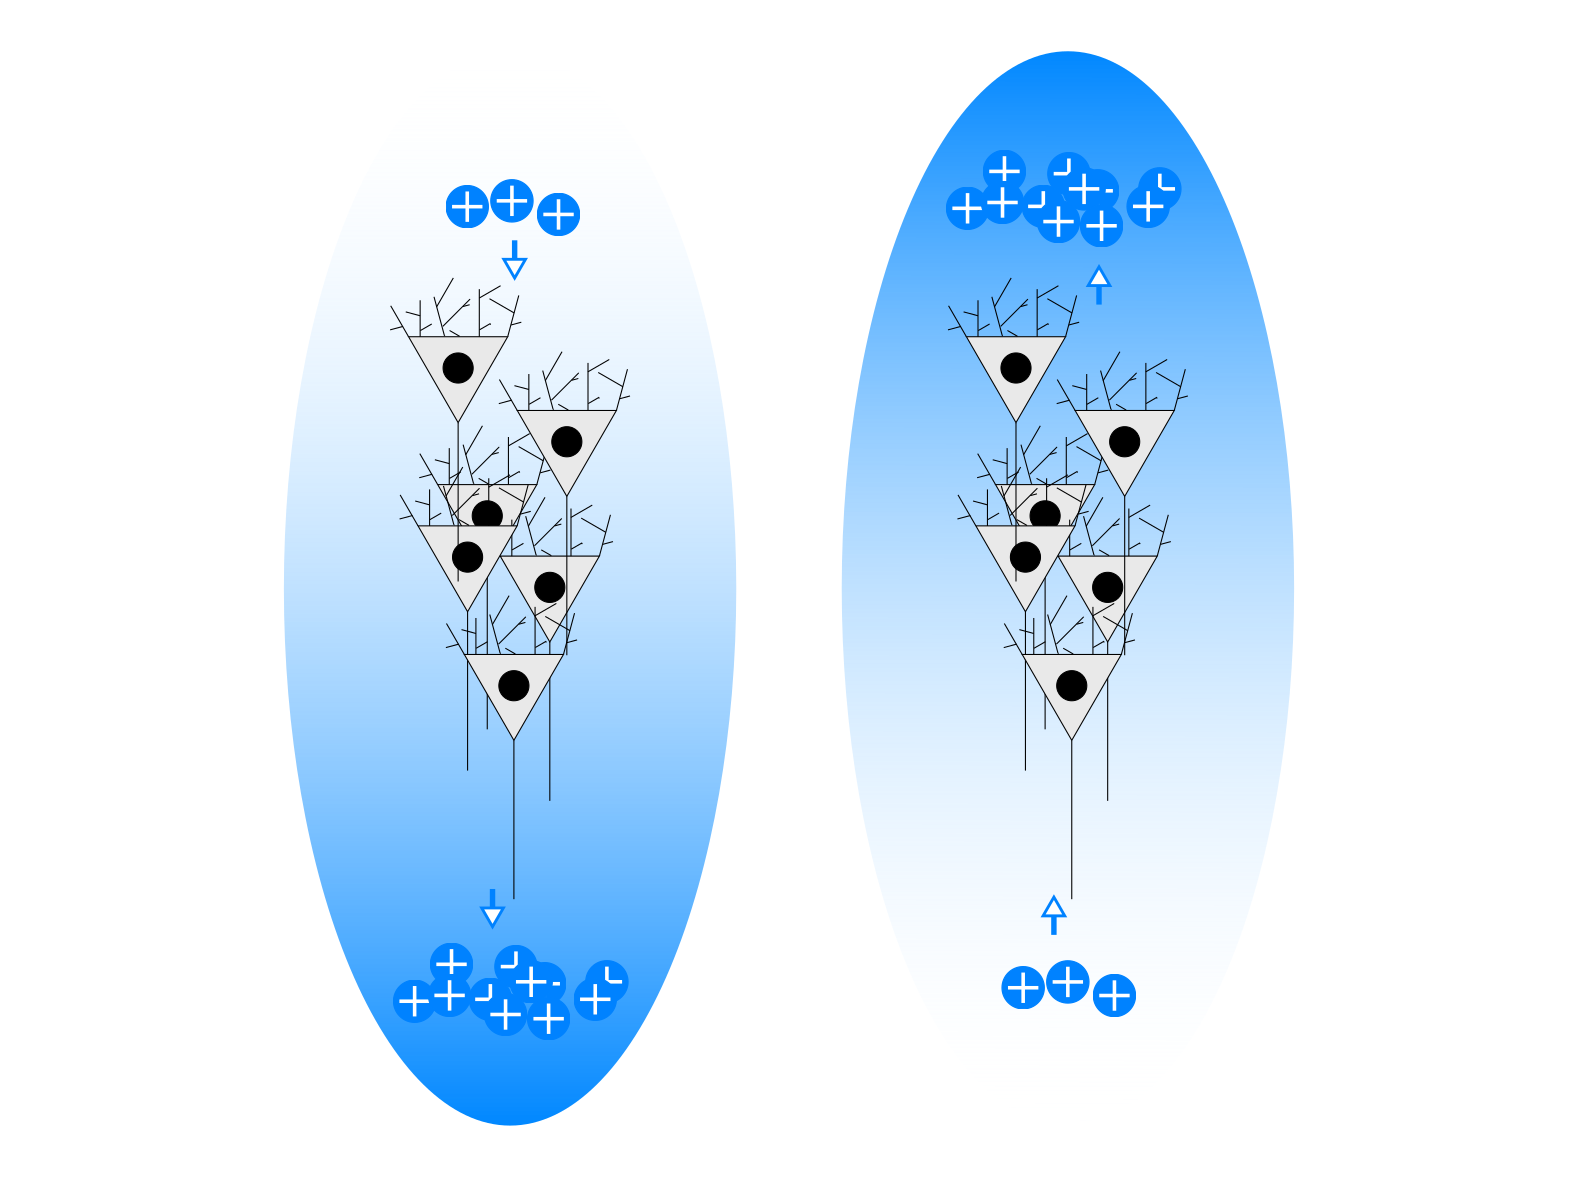
\includegraphics[width=0.9\linewidth,frame]{Thesis/Manuscript/Images/BodyMatter/Introduction/dipole.png}
    \caption[figure title]{figure title}
    \label{fig.intro1}
\end{figure}




\section{Hypothesis}
\begin{itemize}
    \item[\textbullet] 
\end{itemize}


\section{Objectives}

\subsection{General objective}
\begin{itemize}
    \item[\textbullet] 
\end{itemize}


\subsection{Specific objectives}
\begin{itemize}
    \item[\textbullet] 
    
    \item[\textbullet] 
    \item[\textbullet] 
\end{itemize}





\chapter{Materials and Methods}
\section{Data}

\chapter{Results}
\section{my first results}
\subsection{a particular aspect of my first results}
\chapter{Discussion}

\chapter{Conclusions}

My investigation was woderful. It was such a good thing.

\footnotesize{\printbibliography}

\backmatter

\chapter{Publications}
This thesis produced the following publications:
\begin{itemize}

    \item[]\MakeUppercase{ la cita}
\end{itemize}
\clearpage
\chapter{Funding}
{\noindent This work was funded by XXX.}


\end{refcontext}

\end{document}
